\documentclass[a4paper, 12pt]{article}
% packages
\usepackage{amssymb}
\usepackage[fleqn]{mathtools}
\usepackage{tikz}
\usepackage{enumerate}
\usepackage{bussproofs}
\usepackage{xcolor}
\usepackage[margin=1.3cm]{geometry}
\usepackage{logicproof}
\usepackage{diagbox}
\usepackage{listings}
\usepackage{graphicx}
\usepackage{lstautogobble}
\usepackage{hyperref}
\usepackage{multirow}
\usetikzlibrary{arrows, shapes.gates.logic.US, circuits.logic.US, calc, automata, positioning}

% shorthand for verbatim
\catcode`~=\active
\def~#1~{\texttt{#1}}

% code listing
\lstdefinestyle{main}{
    numberstyle=\tiny,
    breaklines=true,
    showspaces=false,
    showstringspaces=false,
    tabsize=2,
    numbers=left,
    basicstyle=\ttfamily,
    columns=fixed,
    fontadjust=true,
    basewidth=0.5em,
    autogobble,
    xleftmargin=3.0ex,
    mathescape=true
}
\newcommand{\dollar}{\mbox{\textdollar}} %
\lstset{style=main}

% augmented matrix
\makeatletter
\renewcommand*\env@matrix[1][*\c@MaxMatrixCols c]{%
\hskip -\arraycolsep
\let\@ifnextchar\new@ifnextchar
\array{#1}}
\makeatother

% ceiling / floor
\DeclarePairedDelimiter{\ceil}{\lceil}{\rceil}
\DeclarePairedDelimiter{\floor}{\lfloor}{\rfloor}

% custom commands
\newcommand{\indefint}[2]{\int #1 \, \mathrm{d}#2}
\newcommand{\defint}[4]{\int_{#1}^{#2} #3 \, \mathrm{d}#4}
\newcommand{\dif}[2]{\frac{\mathrm{d}#1}{\mathrm{d}#2}}
\newcommand{\limit}[2]{\displaystyle{\lim_{#1 \to #2}}}
\newcommand{\summation}[3]{\sum\limits_{#1}^{#2} #3}
\newcommand{\intbracket}[3]{\left[#3\right]_{#1}^{#2}}

\newcommand{\powerset}[0]{\wp}
\renewcommand{\emptyset}[0]{\varnothing}

\newcommand{\unaryproof}[2]{\AxiomC{#1} \UnaryInfC{#2} \DisplayProof}
\newcommand{\binaryproof}[3]{\AxiomC{#1} \AxiomC{#2} \BinaryInfC{#3} \DisplayProof}
\newcommand{\trinaryproof}[4]{\AxiomC{#1} \AxiomC{#2} \AxiomC{#3} \TrinaryInfC{#4} \DisplayProof}

% no indent
\setlength\parindent{0pt}

% reasoning proofs
\usepackage{ltablex}
\usepackage{environ}
\keepXColumns
\NewEnviron{reasoning}{
    \begin{tabularx}{\textwidth}{rlX}
        \BODY
    \end{tabularx}
}
\newcommand{\proofline}[3]{$(#1)$ & $#2$ & \hfill #3 \smallskip \\}
\newcommand{\proofarbitrary}[1]{& take arbitrary $#1$ \smallskip \\}
\newcommand{\prooftext}[1]{\multicolumn{3}{l}{#1} \smallskip \\}
\newcommand{\proofmath}[3]{$#1$ & = $#2$ & \hfill #3 \smallskip \\}
\newcommand{\prooftherefore}[1]{& $\therefore #1$ \smallskip \\}
\newcommand{\proofbc}[0]{\prooftext{\textbf{Base Case}}}
\newcommand{\proofis}[0]{\prooftext{\textbf{Inductive Step}}}

% reasoning er diagrams
\newcommand{\nattribute}[4]{
    \node[draw, state, inner sep=0cm, minimum size=0.2cm, label=#3:{#4}] (#1) at (#2) {};
}
\newcommand{\mattribute}[4]{
    \node[draw, state, accepting, inner sep=0cm, minimum size=0.2cm, label=#3:{#4}] (#1) at (#2) {};
}
\newcommand{\dattribute}[4]{
    \node[draw, state, dashed, inner sep=0cm, minimum size=0.2cm, label=#3:{#4}] (#1) at (#2) {};
}
\newcommand{\entity}[3]{
    \node[] (#1-c) at (#2) {#3};
    \node[inner sep=0cm] (#1-l) at ($(#1-c) + (-1, 0)$) {};
    \node[inner sep=0cm] (#1-r) at ($(#1-c) + (1, 0)$) {};
    \node[inner sep=0cm] (#1-u) at ($(#1-c) + (0, 0.5)$) {};
    \node[inner sep=0cm] (#1-d) at ($(#1-c) + (0, -0.5)$) {};
    \draw
    ($(#1-c) + (-1, 0.5)$) -- ($(#1-c) + (1, 0.5)$) -- ($(#1-c) + (1, -0.5)$) -- ($(#1-c) + (-1, -0.5)$) -- cycle;
}
\newcommand{\relationship}[3]{
    \node[] (#1-c) at (#2) {#3};
    \node[inner sep=0cm] (#1-l) at ($(#1-c) + (-1, 0)$) {};
    \node[inner sep=0cm] (#1-r) at ($(#1-c) + (1, 0)$) {};
    \node[inner sep=0cm] (#1-u) at ($(#1-c) + (0, 1)$) {};
    \node[inner sep=0cm] (#1-d) at ($(#1-c) + (0, -1)$) {};
    \draw
    ($(#1-c) + (-1, 0)$) -- ($(#1-c) + (0, 1)$) -- ($(#1-c) + (1, 0)$) -- ($(#1-c) + (0, -1)$) -- cycle;
}

% actual document
\begin{document}
    \section*{CO130 - Databases}
        \subsection*{Prelude}
            The content discussed here is part of CO130 - Databases (Computing MEng); taught by Thomas Heinis, in Imperial College London during the academic year 2018/19. The notes are written for my personal use, and have no guarantee of being correct (although I hope it is, for my own sake).
        \subsection*{Material Order}
            These notes are primarily based off the slides on CATe. This is the order in which they are uploaded (and I'd assume the order in which they are taught).
            \begin{enumerate}[1.]
                \itemsep0em
                \item \textit{Introduction.pdf}
                \item \textit{ER Modelling.pdf}
                \item \textit{ER to RM.pdf}
                \item \textit{Relational Algebra.pdf}
                \item \textit{Tutorial ER.pdf}
                \item \textit{Tutorial Translation.pdf}
                \item \textit{Relational Algebra.pdf}
                \item \textit{Functional Dependencies.pdf}
                \item \textit{Tutorial Relational Algebra.pdf}
                \item \textit{Normalisation.pdf}
                \item \textit{SQL.pdf}
                \item \textit{Data Definition.pdf}
                \item \textit{Data Manipulation.pdf}
                \item \textit{Advanced SQL.pdf}
                \item \textit{Functional Dependency Tutorial.pdf}
                \item \textit{Transactions.pdf}
                \item \textit{SQL Tutorial.pdf}
                \item \textit{Storage.pdf}
                \item \textit{Indexing.pdf}
                \item \textit{NoSQL.pdf}
                \item \textit{MapReduce.pdf}
            \end{enumerate}
        \subsection*{Introduction}
            We use databases as it's more organised; hence it's easier to model and manage. It's more efficient, as it's fast to search, and update, and integration allows us to minimise data duplication. Concurrent (and therefore multi-user) access allows multiple people to access the database at the same time (will require some techniques).
            \medskip

            \textbf{Transactions} are sequences of database actions that execute in a coherent, and reliable way - the classical properties are \textbf{ACID}. Consider the two transactions ~T1~: $A = A - 100; B = B + 100$, and ~T2~: $B = B - 100; A = A + 100$, we can observe ACID properties as follows;
            \begin{itemize}
                \itemsep0em
                \item \textbf{atomicity} \hfill if one part of a transaction fails, the entire transaction fails
                    \subitem on completion of ~T1~, either $A^\prime = A - 100$, and $B^\prime = B + 100$, or $A^\prime = A$, and $B^\prime = B$, where the former is a successful transaction, and the latter is in the case of a failure.
                \item \textbf{consistency} \hfill transactions don't leave the database in an inconsistent state
                    \subitem the sum of the balances must remain the same, such that $A^\prime + B^\prime = A + B$; we can also have more constraints such as keeping balances positive, or limiting the amount a transfer can do at once
                \item \textbf{isolation} \hfill transactions run as if no other transactions are running (may need to wait)
                    \subitem given the two concurrent transactions ~T1~, and ~T2~, one has to be completed before the other can start
                \item \textbf{durability} \hfill results of successful transactions aren't lost on system failure
                    \subitem the new values, $A^\prime$, and $B^\prime$ must persist if the transaction completes, even if the system fails (disk failure etc.)
            \end{itemize}
            A \textbf{Database Management System (DMBS)} creates new databases via a \textbf{Data Definition Language (DDL)}, which specifies the structure (\textbf{schema}). It also queries, and manipulates through a \textbf{Data Manipulation Language (DML)}. Examples of this include \textit{PostgreSQL}, \textit{MySQL}, \textit{SQLite}, and can also fall under \textit{NoSQL}, however SQL remains as the most widespread technology (as of writing this).
            \medskip

            It lets us define, query, and manipulate databases with a high-level declarative language (\textbf{Structured Query Language}). It's standardised by the ISO, but each DBMS implements its own variation of the standards, which may be costly if it's complex.
            \subsubsection*{Relational Model}
                Consider the following model, represented as a table;
                \begin{center}
                    \begin{tabular}{|c|c|c|c|c|}
                        \hline
                        heading & ~title:string~ & ~year:int~ & ~length:int~ & ~genre:string~ \\
                        \hline
                        \hline
                        \multirow{3}{*}{body} & Gone with the Wind & 1939 & 231 & Drama \\
                        \cline{2-5}
                        & Star Wars & 1977 & 124 & Science Fiction \\
                        \cline{2-5}
                        & Wayne's World & 1992 & 95 & Comedy \\
                        \hline
                    \end{tabular}
                \end{center}
                We have the columns be the attribute, with the top row being the heading, and the rest being the body. The attributes are in the format ~name:type~. The rows (of the body) are referred to as tuples. A relation is the heading as well as the body (the entire table). The heading is an \textbf{unordered set} of attributes, and an attribute is the name as well as the type (typically indivisible types). The body is an unordered set of tuples, and a tuple is the set of attribute values. The schema is for the entire relation is the name of the relation, and the heading, in this case, we'd have; ~movies(title:string, year:int, length:int, genre:string)~, and a database is a collection of relations. A schema for a database is the schemas for all relations.
                \medskip

                In mathematics, with a set of sets; $S_1, S_2, ..., S_n$, a relation $R$ is a set of tuples $T_1, T_2, ..., T_n$, where $T_k \in S_k$, therefore $R \subset S_1 \times S_2 \times ... \times S_n$. As the idea of relations stems from set theory, it's important to note that the order in which we represent the attributes, and tuples in unimportant. In the Relational model we have \textbf{attributed} tuples, rather than \textbf{ordered}; $R$ is the set of tuples ($A_1:S_1=T_1, ..., A_n:S_n=T_n$), with $T_k \in S_k$. It's important to note that relations aren't 2-dimensional tables, even though it's more convenient to draw it on paper. We should instead consider them as a set of $n$-dimensional values, such that we have (~title:string~=StarWars, ~year:int~=1997, ~length:int~=127, ~genre:string~=ScienceFiction), as a 4-dimensional movie value.
        \subsection*{Entity Relationship Modelling}
            When a new database is being developed, it's important to try and model the real-world situation, instead of trying to refine it into an implementation, such as a relational model. In Entity-Relationship modelling, we try to create a diagram which represents the information needed for the database (the Entity Relationship Diagram). As there is no universally accepting notation for ER diagrams, we will use the following notation;
            \begin{center}
                \begin{tabularx}{\textwidth}{|c|X|c|}
                    \hline
                    type & description & shape \\
                    \hline
                    \hline
                    entity sets & a set of distinguishable entries that share the same set of properties, can be physical (a room etc.), an event (flight, sale, etc.) - they normally correspond to nouns & rectangle \\
                    \hline
                    relationship sets & captures how \textbf{two or more} entity sets are related (e.g. owns, tutors), we can also have more than one relationship set between entity sets, and they can also have a relationship set on the same entity - they sometimes correspond to verbs & diamonds \\
                    \hline
                    attributes & properties of an entity; relationship sets can also have attributes, and primary keys are underlined & small circles \\
                    \hline
                \end{tabularx}
                \vspace{-1.5\baselineskip}
            \end{center}
            The movie example is represented below. Note that I've also extended it to contain different types of complex attributes. You can see that the address field is subdivided into number, and postcode, we have a multi-valued attribute in phones, and a derived attribute in age (can be calculated from date of birth)
            \begin{center}
                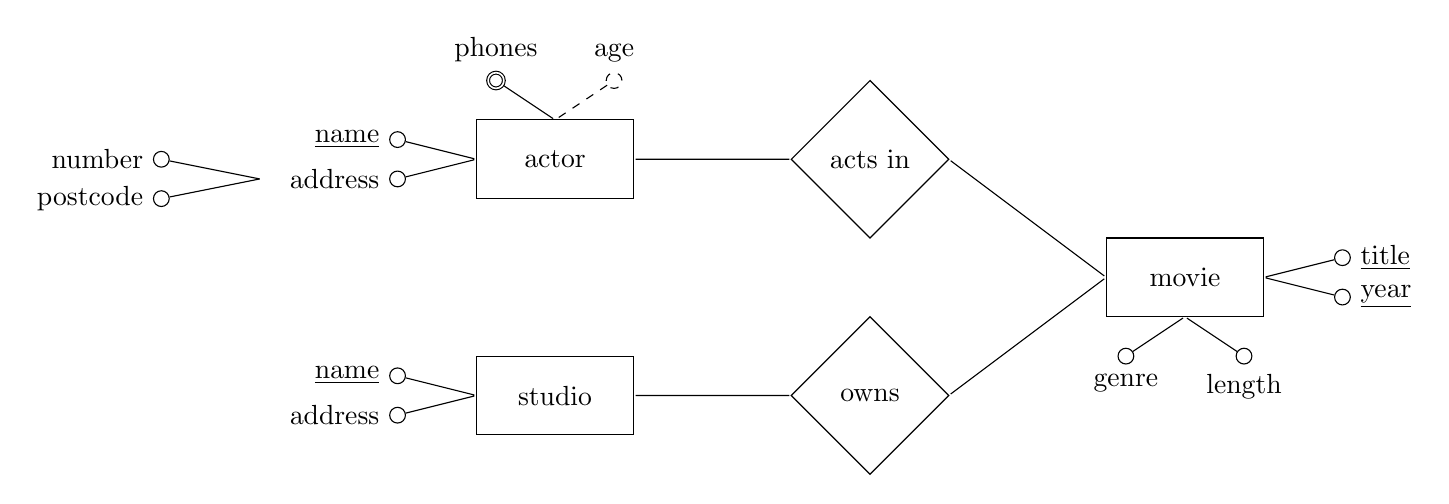
\begin{tikzpicture}
                    \entity{actor}{0, 0}{actor}
                    \entity{studio}{0, -3}{studio}
                    \relationship{actsin}{4, 0}{acts in}
                    \relationship{owns}{4, -3}{owns}
                    \entity{movie}{8, -1.5}{movie}
                    \nattribute{nactor}{-2, 0.25}{left}{\underline{name}}
                    \nattribute{aactor}{-2, -0.25}{left}{address}
                    \mattribute{phones}{-0.75, 1}{above}{phones}
                    \dattribute{age}{0.75, 1}{above}{age}
                    \nattribute{nstudio}{-2, -2.75}{left}{\underline{name}}
                    \nattribute{astudio}{-2, -3.25}{left}{address}
                    \nattribute{mtitle}{10, -1.25}{right}{\underline{title}}
                    \nattribute{myear}{10, -1.75}{right}{\underline{year}}
                    \nattribute{mgenre}{7.25, -2.5}{below}{genre}
                    \nattribute{mlength}{8.75, -2.5}{below}{length}
                    \nattribute{anumber}{-5, 0}{left}{number}
                    \nattribute{apostcode}{-5, -0.5}{left}{postcode}
                    \draw
                    (nactor) -- (actor-l)
                    (aactor) -- (actor-l)
                    (phones) -- (actor-u)
                    (age) edge[dashed] (actor-u)
                    (nstudio) -- (studio-l)
                    (astudio) -- (studio-l)
                    (actor-r) -- (actsin-l)
                    (studio-r) -- (owns-l)
                    (actsin-r) -- (movie-l)
                    (owns-r) -- (movie-l)
                    (movie-r) -- (mtitle)
                    (movie-r) -- (myear)
                    (movie-d) -- (mgenre)
                    (movie-d) -- (mlength)
                    (anumber) -- (-3.75, -0.25)
                    (apostcode) -- (-3.75, -0.25);
                \end{tikzpicture}
            \end{center}
            \subsubsection*{Cardinality Constraints}
                A relationship between two entity sets can be seen as one of the following (using the car example, where a person can drive $N$ cars, and a car can be driven by $M$ people);
                \begin{itemize}
                    \itemsep0em
                    \item one-to-one \hfill $M = 1, N = 1$
                    \item one-to-many \hfill $M = 1$
                    \item many-to-many \hfill no restrictions
                \end{itemize}
                \begin{center}
                    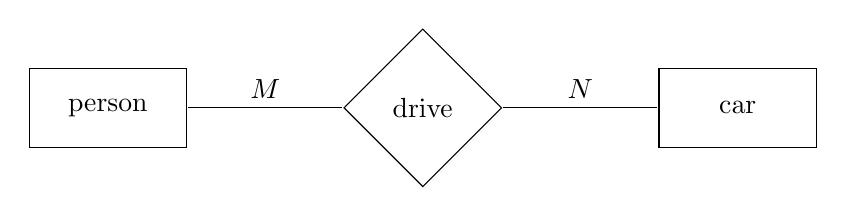
\begin{tikzpicture}
                        \entity{p}{0, 0}{person}
                        \relationship{d}{4, 0}{drive}
                        \entity{c}{8, 0}{car}
                        \draw
                        (p-r) edge[above] node{$M$} (d-l)
                        (d-r) edge[above] node{$N$} (c-l);
                    \end{tikzpicture}
                \end{center}
            \subsubsection*{Participation}
                Using the same example, we can force participation, which means that all entities must participate in a relationship, with a double line. The example below, with the cars, suggests that everyone drives at least 1 car, and car can have at most 1 driver (note that it doesn't mean that every car has a driver).
                \begin{center}
                    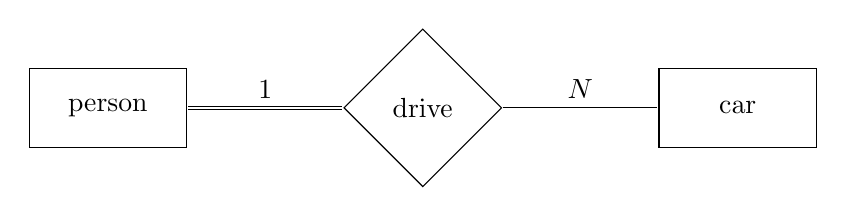
\begin{tikzpicture}
                        \entity{p}{0, 0}{person}
                        \relationship{d}{4, 0}{drive}
                        \entity{c}{8, 0}{car}
                        \draw
                        (p-r) edge[double, above] node{1} (d-l)
                        (d-r) edge[above] node{$N$} (c-l);
                    \end{tikzpicture}
                \end{center}
                Sometimes, instead of using double lines, E-R notation may allow explicit bounds. The below diagram suggests that staff work in exactly 1 branch, and that each branch must have at least 3 members of staff;
                \begin{center}
                    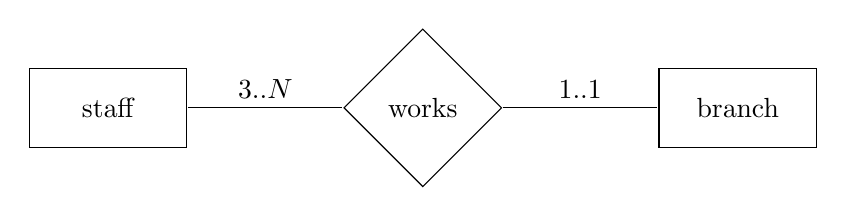
\begin{tikzpicture}
                        \entity{p}{0, 0}{staff}
                        \relationship{d}{4, 0}{works}
                        \entity{c}{8, 0}{branch}
                        \draw
                        (p-r) edge[above] node{$3..N$} (d-l)
                        (d-r) edge[above] node{$1..1$} (c-l);
                    \end{tikzpicture}
                \end{center}
            \subsubsection*{Fan, and Chasm Traps}
                See the diagrams in \textit{ER Modelling.pdf} for examples.
                \medskip

                We need to ensure that we do not allow ambiguous paths between entities. For example, if we say ~staff~ works for ~faculty~ which operates ~department~, if some member of staff works for Engineering, which operates both Computing, and EE, we can't follow a path from the staff member to their department. This can be solved by having the staff work for the department, which is operated by some faculty.
                \medskip

                If we can't follow a path between two entities, we may need to add another relation between them to specify the relationship.
            \subsubsection*{Weak Entities}
                Entities which cannot be uniquely identified by their own attributes are called \textbf{weak} entities, in contrast to \textbf{strong} entities which have primary keys. A weak entity has to be defined by a string entity. Weak entities are drawn as a double rectangle, and the relationship to the strong entity is drawn as a double diamond. The key for a weak entity is formed by combining the primary key of the strong entity with attributes of the weak entity (denoted by a dashed underline). For example, a room in a building is a \textbf{weak} entity, with a room number, and can be uniquely identified with the name of the building combined with the room number.
        \subsection*{ER to RM}
            Keys are used to join information when we do queries. The primary key is the unique identifier of a tuple, and a foreign key is the primary key of \textbf{another} table.
            \medskip

            Once we have an Entity Relationship Model, we can then map it to a relational schema. The schemas can then be refined with functional dependencies, and implemented with relational languages. A high level data model isn't the only concern for database design (considered a simpler aspect).
            \medskip

            If we consider a strong entity set, with simple attributes, we can easily create a table from it (see the example, ~movie~, drawn above).
            \begin{lstlisting}
                movie($\underline{~title~}$, $\underline{~year~}$, length, genre)

                create table movie {
                  title varchar(120),
                  year int,
                  length int,
                  genre char(20),

                  primary key(title, year)
                }
            \end{lstlisting}
            Composite attributes are also fairly easy to represent, since we just flatten it, therefore store each of the sub-attributes as their own field - consider the actor example (note that if the primary key is composite, we mark all the sub-attributes as primary keys). This example also shows how multi-valued attributes are stored - we create their own relation, and link back to the entity set with a foreign key constraint;
            \begin{lstlisting}
                actor($\underline{~name~}$, number, postcode)
                actor_phones($\underline{~actorName~}$, $\underline{~phoneID~}$, $\textit{~other attributes~}$)

                create table actor {
                  name varchar(60),
                  number int,
                  postcode varchar(10),

                  primary key (name)
                }

                create table actor_phones {
                  actorName varchar(60),
                  phoneID varchar(10),
                  ...
                  primary key (actorName, phoneID),
                  foreign key (actorName) references actor.name
                }
            \end{lstlisting}
            The relational model doesn't allow us to specify derived attributes, and we're therefore expected to calculate them with queries.
            \medskip

            We can also consider how many-to-many relationships can be represented (using the car example again). The first example is when a car can be driven by many people, and a person can drive many cars;
            \begin{lstlisting}
                person($\underline{~ID~}$, $\textit{~other attributes~}$)
                car($\underline{~regno~}$, $\textit{~other attributes~}$)
                drive($\underline{~personID~}$, $\underline{~regno~}$, $\textit{~other attributes~}$)

                create table drive {
                  personID varchar(10),
                  regno varchar(12),
                  ...
                  primary key (personID, regno),
                  foreign key (personID) references person.ID on delete cascade,
                  foreign key (regno) references car.regno on delete cascade
                }
            \end{lstlisting}
            However, it's easier to represent a one-to-many relationship, as we can simply include the primary key of the "one" relation as a foreign key in the many (where a car can be driven by 1 person, and a person can drive many cars). The representation for a one-to-one is similar, but the foreign key can be in either one, which is up to the designer;
            \begin{lstlisting}
                person($\underline{~ID~}$, $\textit{~other attributes~}$)
                car($\underline{~regno~}$, personID, $\textit{~other attributes~}$)

                create table car {
                    regno varchar(12),
                    personID varchar(10),
                    ...
                    primary key (regno),
                    foreign key (personID) references person.ID
                }
            \end{lstlisting}
            In a weak entity, we include the primary key of the strong relation as a foreign key, but also use it as part of the composite primary key for the weak entity. A delete cascade is also used, and finally the we use ~not null~ to ensure total participation;
            \begin{lstlisting}
                building($\underline{~name~}$, $\textit{~other attributes~}$)
                room($\underline{~no~}$, $\underline{~buildingname~}$, $\textit{~other attributes~}$)

                create table room {
                    no varchar(120),
                    buildingname varchar(50) not null,
                    ...
                    primary key (no, buildingname),
                    foreign key (buildingname) references building.name on delete cascade
                }
            \end{lstlisting}
            A multiway relationship can be mapped as several binary relationships, or we can generalise it to have the primary key consist of the relationship be composed of the primary keys of the many entity sets, and have the primary keys of the one entities be attributes. For roles, we map each role as a foreign key attribute in the entity set;
            \begin{lstlisting}
                movie($\underline{~ID~}$, $\textit{~other attributes~}$)
                sequelof($\underline{~originalID~}$, $\underline{~sequelID~}$, $\textit{~other attributes~}$)

                create table sequelof {
                    originalID int,
                    sequelID int,
                    ...
                    primary key (orignalID, sequelID),
                    foreign key originalID references movie.ID,
                    foreign key sequelID references movie.ID
                }
            \end{lstlisting}
            \subsubsection*{Extended Models}
                Newer models extend the classic model by supporting features from \textbf{object-oriented design}. We can look at how E-R models handle specialisation, or generalisation with \textbf{is-a hierarchies}. For example, we can specify that a ~cartoon~ \textbf{is-a} ~movie~, which means that it inherits all the attributes of movie, but can have more attributes. and relations. Once this extends on multiple levels, we begin to form a hierarchy.
        \subsection*{Relational Algebra}
            We can use \textbf{relational algebra} to construct new relations from existing ones, the operators include selection, projection, intersection, union, difference, and product. Consider the examples below, ~a~, ~b~, and ~c~ are all integers. Intersection, union, and difference will be omitted, since those are fairly self-explanatory.
            \begin{center}
                \begin{tabular}{|cccccc|ccc|ccc|ccc|}
                    \hline
                    \multicolumn{6}{|c|}{$R$} & \multicolumn{3}{c|}{$\pi_{~a,c,e~}(R)$} & \multicolumn{3}{c|}{$S$} & \multicolumn{3}{c|}{$\sigma_{~a>3|b<5~}(S)$} \\
                    \hline
                    ~a~ & ~b~ & ~c~ & ~d~ & ~e~ & ~f~ & ~a~ & ~c~ & ~e~ & ~a~ & ~b~ & ~c~ & ~a~ & ~b~ & ~c~ \\
                    \hline
                    1 & 2 & 3 & 4 & 5 & 6 & 1 & 3 & 5 & 3 & 2 & 3 & 3 & 2 & 3 \\
                    1 & 1 & 1 & 1 & 1 & 1 & 1 & 1 & 1 & 2 & 1 & 7 & 8 & 2 & 2 \\
                    2 & 2 & 2 & 2 & 2 & 2 & 2 & 2 & 2 & 8 & 2 & 2 & & & \\
                    1 & 2 & 3 & 4 & 5 & 8 & & & & 1 & 2 & 9 & & & \\
                    \hline
                \end{tabular}
            \end{center}
            The syntax in use here for projection is $\pi_{~attributes~}(T)$, and likewise for selection it's $\sigma_{~condition~}(T)$. The former returns a relation with only the listed attributes, and the only takes rows which satisfy the given condition. Neither will return duplicate rows. Here is an example of a Cartesian product;
            \begin{center}
                \begin{tabular}{|cc|ccc|ccccc|}
                    \hline
                    \multicolumn{2}{|c|}{$R$} & \multicolumn{3}{c|}{$S$} & \multicolumn{5}{c|}{$R \times S$} \\
                    \hline
                    ~a~ & ~b~ & ~c~ & ~d~ & ~e~ & ~a~ & ~b~ & ~c~ & ~d~ & ~e~ \\
                    \hline
                    1 & 2 & 1 & 2 & 3 & 1 & 2 & 1 & 2 & 3 \\
                    3 & 4 & 4 & 5 & 6 & 1 & 2 & 4 & 5 & 6 \\
                    & & 7 & 8 & 9 & 1 & 2 & 7 & 8 & 9 \\
                    & & & & & 3 & 4 & 1 & 2 & 3 \\
                    & & & & & 3 & 4 & 4 & 5 & 6 \\
                    & & & & & 3 & 4 & 7 & 8 & 9 \\
                    \hline
                \end{tabular}
            \end{center}
            We can take a natural join, where the resulting relation contains all the tuples that have matching attributes in $R$, and $S$. This is less common, and we'd typically use something closer to $R \bowtie_{R.~b~ = S.~b~} S$. Note that in this case, they are the same, since that's the only attribute that overlaps;
            \begin{center}
                \begin{tabular}{|cc|ccc|cccc|}
                    \hline
                    \multicolumn{2}{|c|}{$R$} & \multicolumn{3}{c|}{$S$} & \multicolumn{4}{c|}{$R \bowtie S$} \\
                    \hline
                    ~a~ & ~b~ & ~b~ & ~c~ & ~d~ & ~a~ & ~b~ & ~c~ & ~d~ \\
                    \hline
                    1 & 2 & 1 & 2 & 3 & 1 & 2 & 5 & 6 \\
                    1 & 3 & 2 & 5 & 6 & 3 & 4 & 8 & 9 \\
                    3 & 4 & 4 & 8 & 9 & 3 & 4 & 9 & 9 \\
                    & & 4 & 9 & 9 & & & & \\
                    \hline
                \end{tabular}
            \end{center}
            Attributes can also be renamed with the notation $\rho_{~new/old~, ...}(R)$ notation, which is fairly self-explanatory.
        \subsection*{Functional Dependencies}
            Relational database schemas should be normalised, which helps reduce redundancy, and avoids update, and deletion anomalies. The basis for normalisation is the concept of \textbf{functional dependency}, and \textbf{keys}. Consider the following example, which can experience update anomalies;
            \begin{center}
                \begin{tabular}{|l|l|l|l|l|}
                    \hline
                    producer & city & product no. & price & quantity \\
                    \hline
                    \hline
                    3 & London & 52 & 65 & 4 \\
                    22 & Birmingham & 10 & 15 & 5 \\
                    22 & Birmingham & 12 & 4 & 11 \\
                    3 & London & 44 & 43 & 32 \\
                    3 & London & 43 & 3 & 27 \\
                    \hline
                \end{tabular}
            \end{center}
            If an existing producer changes address, and tuples aren't updated, then it leads to incoherence (as the data would now be invalid). If a new tuple / row is inserted, and the producer already exists, but with an older address, we will once again have incoherence. If a producer doesn't have any open orders, say rows 1, and 5 didn't exist, then data about producer 3 would be lost. The price of the product doesn't depend on the producer, and the location of the producer doesn't have anything to do with the product. There is also redundant data, since the address is duplicated. Ideally, the data should be stored like this;
            \begin{center}
                \begin{minipage}[t]{0.4\textwidth}
                    \begin{tabular}{|l|l|l|}
                        \hline
                        \multicolumn{3}{|l|}{Open Orders} \\
                        \hline
                        producer no. & product no. & quantity \\
                        \hline
                        \hline
                        3 & 52 & 4 \\
                        22 & 10 & 5 \\
                        22 & 12 & 11 \\
                        3 & 44 & 32 \\
                        3 & 43 & 27 \\
                        \hline
                    \end{tabular}
                \end{minipage}
                \begin{minipage}[t]{0.3\textwidth}
                    \begin{tabular}{|l|l|}
                        \hline
                        \multicolumn{2}{|l|}{Producer} \\
                        \hline
                        producer no. & city \\
                        \hline
                        \hline
                        3 & London \\
                        22 & Birmingham \\
                        & \\
                        & \\
                        & \\
                        \hline
                    \end{tabular}
                \end{minipage}
                \begin{minipage}[t]{0.21\textwidth}
                    \begin{tabular}{|l|l|}
                        \hline
                        \multicolumn{2}{|l|}{Product} \\
                        \hline
                        product no. & price \\
                        \hline
                        \hline
                        52 & 65 \\
                        10 & 15 \\
                        12 & 4 \\
                        44 & 43 \\
                        43 & 3 \\
                        \hline
                    \end{tabular}
                \end{minipage}
            \end{center}
            A functional dependency is a constraint that if two tuples of a relation $R$ agree on a set of attributes $A_1, A_2, ..., A_n$, then they must also agree on the set of attributes $B_1, B_2, ..., B_m$. This can be written as $A_1, A_2, ..., A_n \rightarrow B_1, B_2, ..., B_m$, and therefore the $B$ set is functionally dependant on the $A$ set, or the $A$ set functionally determines the $B$ set. Therefore, for any set of values $A$, then there is only one set of values $B$. The normal forms a designer can use are defined in terms of their functional dependencies. This can be summarised by the following examples;
            \begin{center}
                \begin{tabular}{|c|c|c|}
                    \hline
                    functional dependency & for all tuple pairs, $x$, $y$, if & then assert \\
                    \hline
                    $A \rightarrow K$ & $x.A = y.A$ & $x.K = y.K$ \\
                    \hline
                    $A, B \rightarrow K$ & $x.A = y.A$ & $x.K = y.K$ \\
                    & $x.B = y.B$ & \\
                    \hline
                    $A \rightarrow K, L$ & $x.A = y.A$ & $x.K = y.K$ \\
                    & & $x.L = y.L$ \\
                    \hline
                    $A, B \rightarrow K, L$ & $x.A = y.A$ & $x.K = y.K$ \\
                    & $x.B = y.B$ & $x.L = y.L$ \\
                    \hline
                \end{tabular}
            \end{center}
            Note that if we have two functional dependencies, $A, B \rightarrow K$, and $A, B \rightarrow L$, it's trivial to combine them as $A, B \rightarrow K, L$ (or to split them). If we have the functional dependency $A, B, C, D, E \rightarrow A, C, X, Y, Z$, we can remove all the attributes on the right hand side, that are on the left hand side, such that the aforementioned FD reduces to $A, B, C, D, E \rightarrow X, Y, Z$. A \textbf{trivial} FD is one where all the attributes on the RHS are on the LHS.
            \subsubsection*{Keys}
                If we have some set of attributes $A_1, A_2, ..., A_n$, functionally determine all the remaining attributes of the relation, then the set $A$ is a \textbf{superkey}. This also implies that two tuples cannot have the same superkey values, due to the uniqueness property. Let there be a set of all attributes in the relation, $K$, and the superkey set $S$. Therefore we can state $S \rightarrow \{ x \in K\ |\ x \notin S \}$. A single relation may have more than one superkey, and superkeys can contain attributes that aren't strictly required. Generally, we are interested in superkeys where there isn't a subset of the superkey (hence the smallest superkey, by the irreducibility property), and this minimal superkey is referred to as the \textbf{candidate key}. If we have more than one candidate key, we can choose one of them to act as the primary key.
            \subsubsection*{Closure}
                The set of all attributes functionally determined by a set $L$, under a set of dependencies $F$, the closure of $L$, denoted as $L^+$. If $L^+$ contains all the attributes of $R$, then it follows that $L$ is a superkey of $R$. If $\text{RHS} \subseteq \text{LHS}^+$, then $\text{LHS} \rightarrow \text{RHS}$ holds.
                \medskip

                In order to compute the closure of a set of attributes, $L$, under a set of FDs given in the form $\text{LHS} \rightarrow \text{RHS}$, we keep adding all the LHSs which exist as a subset of $L$, and add the RHS to $L$. We repeat this until we can no longer add anymore RHSs. The final value is referred to as $L^+$. Given the starting value of $L = \{A, B\}$, and the following FD set;
                \begin{enumerate}[(1)]
                    \itemsep0em
                    \item $A, B \rightarrow C$
                    \item $B, C \rightarrow A, D$
                    \item $D \rightarrow E$
                    \item $C, F \rightarrow B$
                \end{enumerate}
                Starting with (1), both $A$, and $B$ are in $L$, so we can add $C$. Now that $C$ is in $L$, and $B$ was already there, we can add $D$ (no need to add $A$) from (2). Since we have $D$ in $L$, we can add $E$. There is nothing else we can do, since $F$ is not in $L$. Hence the value of $L^+ = \{A, B, C, D, E\}$.
            \subsubsection*{Armstrong's Axioms}
                This is a sound (doesn't generate incorrect FDs), and compete (allows us to derive all valid FDs) axiomisation of FDs. Given attributes $A, B, C, ...$, and sets of attributes $\alpha, \beta, \gamma$, we have the following axioms;
                \begin{itemize}
                    \itemsep0em
                    \item reflexivity (trivial FDs) \hfill $\alpha \rightarrow \beta$ always holds if $\beta \subseteq \alpha$
                    \item augmentation \hfill if $\alpha \rightarrow \beta$, then it follows $\alpha \gamma \rightarrow \beta \gamma$
                    \item transitivity \hfill if $\alpha \rightarrow \beta$, and $\beta \rightarrow \gamma$, then $\alpha \rightarrow \gamma$
                    \item (derived) union \hfill if $\alpha \rightarrow \beta$, and $\alpha \rightarrow \gamma$, then $\alpha \rightarrow \beta \gamma$
                    \item (derived) decomposition \hfill if $\alpha \rightarrow \beta \gamma$, then $\alpha \rightarrow \beta$, and $\alpha \rightarrow \gamma$
                    \item (derived) pseudotransitivity \hfill if $\alpha \rightarrow \beta$, and $\delta \beta \rightarrow \gamma$, then $\delta \alpha \rightarrow \gamma$
                \end{itemize}
            \subsubsection*{Closure, and Covers}
                Similar to attributes, we can find the closure of a FD set, which is the set of all FDs that can be inferred, denoted as $F^+$. This can be approached by applying Armstrong's axioms. We start by initialising $F^+$ to the set $F$. By applying reflexivity, and augmentation, we can add new FDs to $F^+$. Transitivity can then be applied to suitable FDs, and adding the derived ones to $F^+$. This is repeated until no more changes occur.
                \medskip

                We can say two FD sets $F_1$, and $F_2$ are equivalent if they each imply the other - if any relation instance satisfying $F_1$ also satisfies $F_2$, they are said to be covers of each other. A cover is canonical / minimal / irreducible if each LHS is unique, and no FD can be deleted from the cover, and still maintain an equivalent FD set. Additionally, no attributes can be deleted from any FD set, and still have an equivalent set. Therefore, the canonical cover has no redundant dependencies, nor attributes.
                \medskip

                The method for testing whether some attribute, $X$, is extraneous depends on whether it's on the LHS, or RHS. For an attribute $X$ on the LHS, we can say $X$ is extraneous if $\text{RHS} \subseteq \{\text{LHS} - X\}^+$ under the FD set - note that here we are referring to closure on attributes, not FDs. On the other hand (no pun intended, I'm so depressed), an attribute $X$ on the RHS is extraneous if $X \in \text{LHS}^+$ under the FD set, where $X$ is removed from the RHS of all the FDs in the set.
                \medskip

                To compute a canonical cover $F$ for an FD set, we can use the following algorithm;
                \begin{lstlisting}
                    let $F$ := FD set
                    do
                        replace dependencies of $\alpha \rightarrow \beta$ and $\alpha \rightarrow \gamma$, with $\alpha \rightarrow \beta \gamma$
                        remove all extraneous attributes one at a time
                    until $F$ doesn't change
                \end{lstlisting}
        \subsection*{Normalisation}
            As previously mentioned, in the previous section, normalisation reduces data duplication, and anomalies. One of the approaches taken to develop a normalised schema is to start with a few big relations, and then decompose them into a suitable normal form. The ones we'll look at are \textbf{Boyce-Codd Normal Form (BCNF)}, and \textbf{Third Normal Form (3NF)}. Consider the following example, which is just a "big" relation;
            \begin{center}
                \begin{tabular}{|c|c|c|c|c|c|}
                    \hline
                    ~title~ & ~year~ & ~length~ & ~genre~ & ~studio~ & ~actor~ \\
                    \hline
                    \hline
                    Star Wars & 1977 & 124 & Science Fiction & Fox & Carrie Fisher \\
                    \hline
                    Star Wars & 1977 & 124 & Science Fiction & Fox & Mark Hamill \\
                    \hline
                    Star Wars & 1977 & 124 & Science Fiction & Fox & Harrison Ford \\
                    \hline
                    Gone with the Wind & 1939 & 231 & Drama & MGM & Vivien Leigh \\
                    \hline
                    Wayne's World & 1992 & 95 & Comedy & Paramount & Dana Carvey \\
                    \hline
                    Wayne's World & 1992 & 95 & Comedy & Paramount & Mile Myers \\
                    \hline
                \end{tabular}
            \end{center}
            You'll notice straight away that there is a huge amount of redundant, repeated data, which is present in multiple rows. Updating the ~length~ of Star Wars would require 3 updates (for the relation to remain consistent), which is error prone. Inserting a new actor for a movie would require duplicating a fair bit of data, and would require checks to maintain consistency. Finally, deleting Vivien Leigh would delete the entire row, which deletes information about the movie.
            \subsubsection*{Decomposition}
                Given a relation $R(A_1, A_2, ..., A_n)$, we can decompose it into two projected relations $S$, and $T$, such that $\text{attr}(R) = \text{attr}(S) \cup \text{attr}(T)$. This also means that $S = \pi_{\text{attr}(S)}(R)$, and similar for $T$.
                \medskip

                When we decompose a relation, it's crucial for us to ensure we can recover the original relation by joining the decomposed relations, and also preserve the FDs of the original relation. Note that the latter isn't always possible with BCNF.
                \medskip

                Given $R$ decomposed into $S$, and $T$, the decomposition is \textbf{lossless} if at least one of the following FDs hold in the closure of FD set of $R$;
                \begin{itemize}
                    \itemsep0em
                    \item $\text{attr}(S) \cap \text{attr}(T) \rightarrow \text{attr}(S)$
                    \item $\text{attr}(S) \cap \text{attr}(T) \rightarrow \text{attr}(T)$
                    \item this means the common attributes of $S$, and $T$ form a superkey of either of the decomposed relations
                \end{itemize}
                If we're able to check the FDs of $R$ without joining the decomposed sets, then the decomposition is \textbf{dependency preserving}.
                \medskip

                Consider the following example, on $R(A, B, C)$, with the FD set $\{A \rightarrow B, B \rightarrow C\}$;
                \begin{center}
                    \vspace{-\baselineskip}
                    \begin{tabularx}{\textwidth}{|l|l|X|}
                        \hline
                        decomposition & lossless? & dependency preserving? \\
                        \hline
                        $S(A, B)$ & $B \rightarrow A, B$ doesn't hold & yes, $A \rightarrow B$ is checked with $S$, and $B \rightarrow C$ with $T$ \\
                        $T(B, C)$ & $B \rightarrow B, C$ holds $\therefore$ lossless & \\
                        \hline
                        $S(A, B)$ & $A \rightarrow A, B$ holds $\therefore$ lossless & no, $B \rightarrow C$ cannot be checked without joining \\
                        $T(A, C)$ & $A \rightarrow A, C$ holds also & \\
                        \hline
                    \end{tabularx}
                    \vspace{-2\baselineskip}
                \end{center}
            \subsubsection*{Boyce-Codd Normal Form}
                \textbf{A relation $R$ is in BCNF, if and only if, for all non-trivial FDs (including derived FDs) of the relation, the LHS of every FD is a superkey (i.e. contains a key)}
                \bigskip

                For example, if we have the FD $~title~, ~year~ \rightarrow ~length~, ~genre~, ~studio~$, it's not in BCNF, as ~title~, ~year~ doesn't functionally determine ~actor~.
\end{document}
